\label{desenvolvimento_eletroeletronica}

Nesta seção é descrito o detalhamento da solução do módulo de eletroeletrônica, resultante das duas primeiras fases,
e o seu projeto e construção, resultante da Fase 03.

\subsection{Detalhamento de Solução}

\subsubsection*{Desenvolvimento de arquitetura para o sistema de sensoriamento}

A arquitetura do projeto da mesa deve cumprir os seguintes pré-requisitos:

\begin{itemize}
    \item Ser escalável, isto é, comportar um aumento de sensores disponíveis. Para isso, optou-se por sensores interfaceados por I2C, e um sistema baseado em multiplexadores e Registradores de deslocamento para o controle da leitura do sensor.
    \item Garantir a correta frequencia de amostragem para os sensores disponibilizados.
    \item Possuir interface de comunicação externa com qualquer dispositivo que queira controlar parametros de vibração da mesa, como a frequencia.
    \item Possuir a função de “módulo mestre”, controlando todos os demais, e sendo controlado via UART.
\end{itemize}

\subsubsection*{Desenvolvimento de arquitetura para um sistema de controle de motores}

A arquitetura do projeto do módulo de controle de motores deve cumprir os seguintes pré-requisitos:

\begin{itemize}
    \item Ser  controlável via I2C, recebendo e enviando comandos do módulo mestre.
    \item Possuir capacidade de controle em malha fechada da frequencia da mesa.
    \item Possuir capacidade de controle do motor.
\end{itemize}

\subsection{Projeto e construção}

Um módulo BSP é uma coletânia de códigos básicos de microcontrolador, que implementam um a um todas as suas funcionalidades. Dessa forma, funções mais alto nível são disponibilizadas para a aplicação, tornando-a mais genérica e permitindo que a mesma possa suportar mais de um microcontrolador ao mesmo tempo. \\
Para o projeto em questão, as seguintes implementações específicas de MSP430 foram criadas. Todas são suportadas para dois microntoladores (MSP430F2274 e MSP430G25543), de forma que se reduz ao mínimo o tempo de desenvolvimento de código, sem perder a robustez e flexibilidade.

\begin{figure}[htbp]
    \centering
        \includegraphics[scale=0.6]{figuras/bsp.png}
    \caption{Pacotes implementados para o BSP}
    \label{bsp-scheme}
\end{figure}

\subsection*{Sistema Bevim}

O sistema BeVim é composto pelos seguintes módulos:

\begin{itemize}
    \item Módulo de Sensoriamento - Parte responsável pela leitura de sensores, comunicação com a CPU e controle dos módulos de motores.
    \item Módulo de Motor - Parte responsável pelo controle de inversores, e pela retroalimentação em malha fechada para atingir frequencias altas.
\end{itemize}

Ambos os moódulos são conectados entre si por uma rede I2C (InterIntegrated Circuits), onde o módulo de sensoriamento sempre atua como mestre no processo de comunicação. Esse procedimento foi escolhido pela possibilidade de se adicionar de maneira fácil outros módulos (de motor, por exemplo, ou outros que sejam de interesse a serem desenvolvidos), não interferindo com outros sistemas perifericos a mesa.

\subsubsection*{Módulo de Sensoriamento}
O módulo de sensoriamento é o responsável pela implementação da interface (via protocolo BeVim) com o sistema que controla a mesa em alto nível - a CPU. Ao mesmo tempo, esse módulo executa um controle da leitura dos sensores digitais do projeto, e dos outros módulos acoplados (os de motores).

\begin{figure}[htbp]
    \centering
        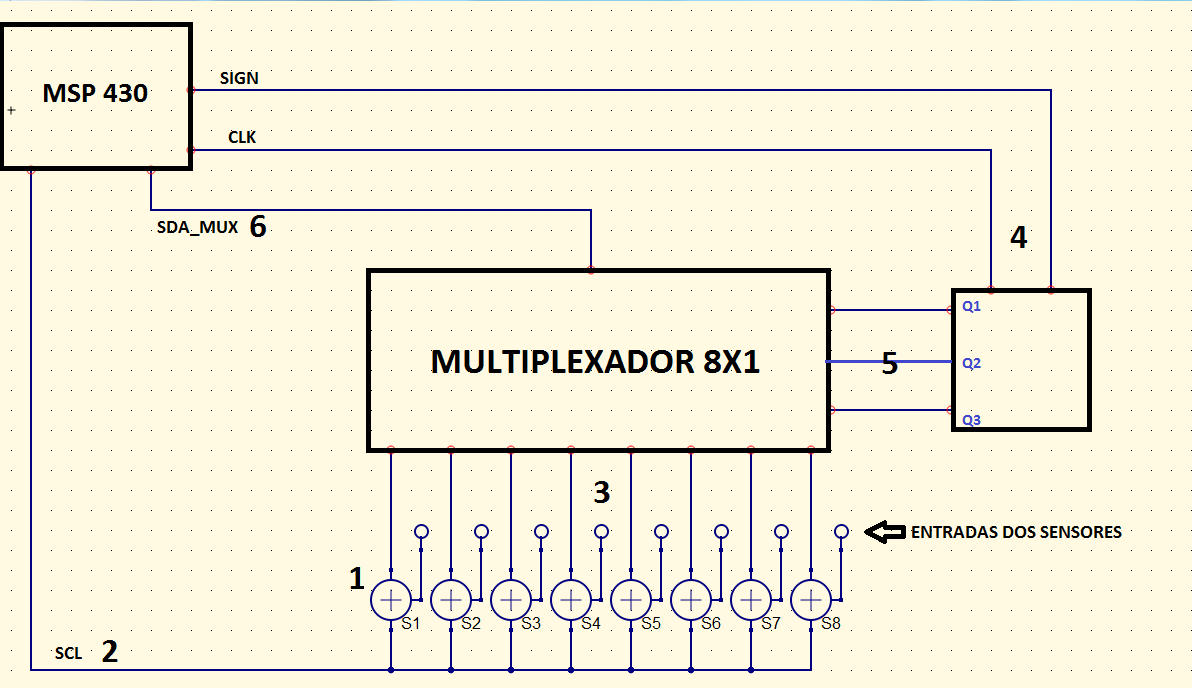
\includegraphics[scale=0.6]{figuras/mod_sensor.png}
    \caption{Módulo de Sensoriamento}
    \label{mod_sensor}
\end{figure}

Itens da Figura \ref{mod_sensor}:

\begin{enumerate}
    \item Conectores DB9, que receptam os sinais dos acelerômetros.
    \item Os sensores recebem sinais de clock provindos do microcontrolador, através do sinal SCL da rede I2C.
    \item Os sinais de dados de cada sensor servem como entrada de um multiplexador 8x1.
    \item O MSP430, através de duas portas GPIO's, controlam um registrador responsável pelas portas seletoras do multiplexador. Uma porta é o sinal serial de seleção “sign” e a outra é o clock “clk”.
    \item O conjunto do registrador com o multiplexador é capaz de selecionar qual sensor será aferido pelo sistema.
    \item O dado do sensor selecionado é enviado para a rede I2C através do caminho SDA-MUX
\end{enumerate}

\subsubsection*{Módulo de Motor}

\begin{figure}[htbp]
    \centering
        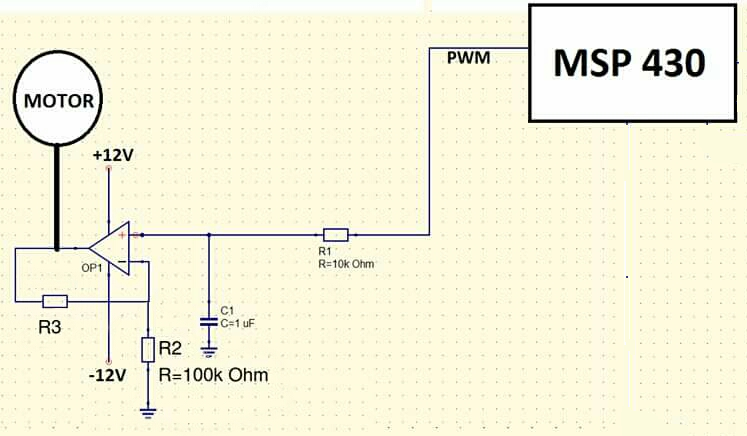
\includegraphics[scale=0.6]{figuras/mod_motor.png}
    \caption{Módulo do Motor}
    \label{mod_motor}
\end{figure}


\subsection*{Circuito Completo}

\begin{figure}[htbp]
    \centering
        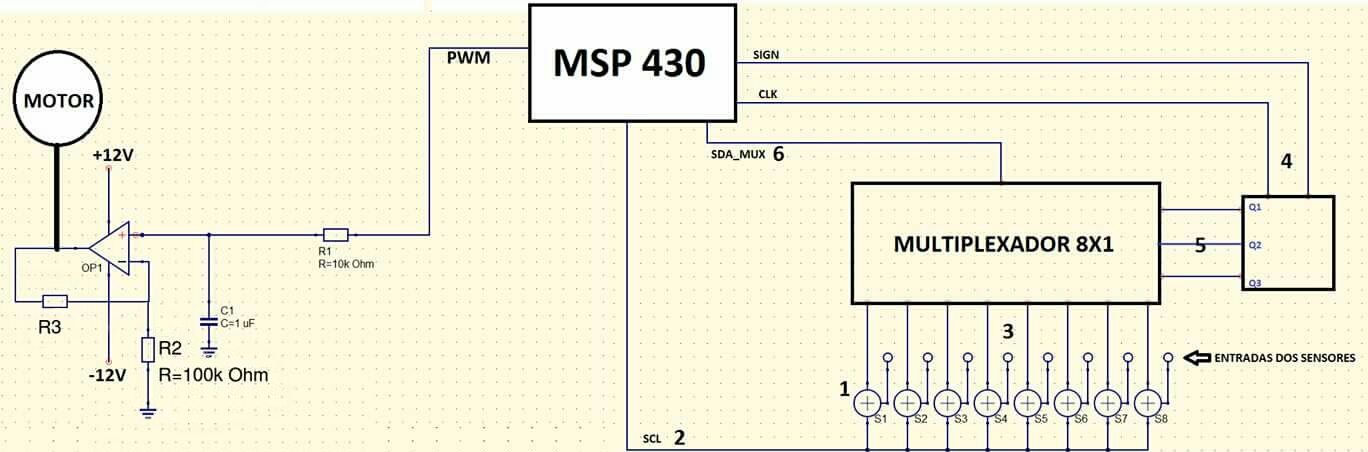
\includegraphics[scale=0.2]{figuras/mod_completo.png}
    \caption{Circuito Completo}
    \label{mod_completo}
\end{figure}

\subsection*{Detecção de Módulos Adicionais}

Um fator importante no sistema é a escalabilidade do mesmo, para que seja resiliente a má operação do usuário e a falhas, se torna necessário a detecção automática de módulos adicionais de sensores. Para a implementação desse mecanismo, sera usado o principio simples do divisor de tensão. Cada modulo possuirá uma resistência de valor igual ao de uma resistência de referencia pre-determinada $R_{ref1}$. O circuito da figura \ref{circ-exp} sera usado para essa função:

\begin{figure}[htbp]
    \centering
        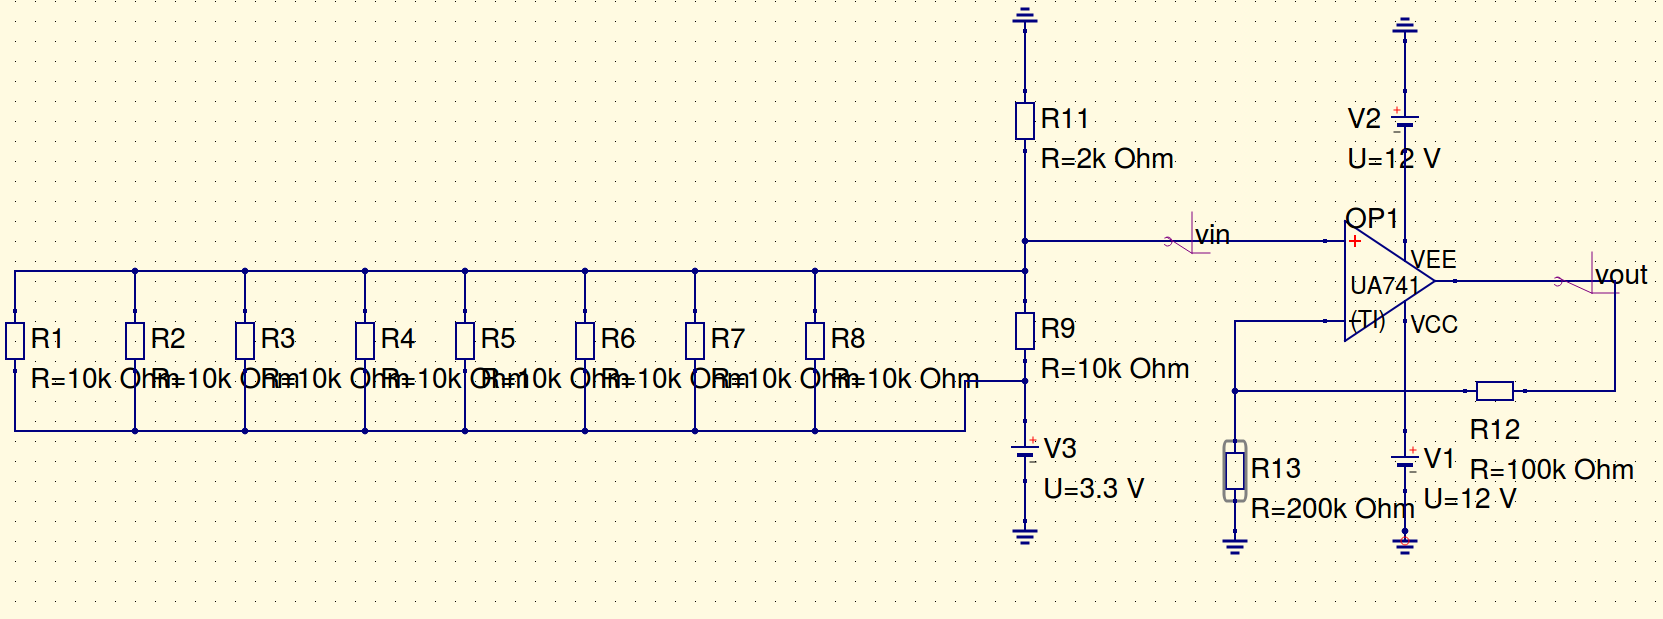
\includegraphics[scale=0.1]{figuras/exp-board-detection.png}
    \caption{Circuito de Expansao}
    \label{circ-exp}
\end{figure}

Os módulos de expansão (representados pelas resistências de $R_{1}$ a $R_{8}$ serão conectados em paralelo e assim a resistência da combinação dos mesmo sera cada vez menor, e consequentemente maior sera a tensão de entrada no amplificador operacional. Essas resistências dos módulos devem ser sempre de valor o mais próximo possível de $R_{ref1}$ para garantir o funcionamento. O amplificador esta na configuração não inversora, e possui ganho representado na equação \ref{ganho-simples}:

\begin{equation}\label{ganho-simples}
A=\frac{ R_{a} }{ R_{b} } + 1
\end{equation}

A resistência equivalente da combinação dos módulos com a resistência de referencia é dado pela equação \ref{resEq}:

\begin{equation}\label{resEq}
ResEq = \left( \frac{ N_{sensores} + 1 }{ R_{ref1} } \right)^{-1}  = \frac{ R_{ref1} }{ N_{sensores} + 1 }
\end{equation}

Consequentemente a tensão de saída sera dada por:

\begin{equation}\label{resEq}
V_{out} = \frac{R_{ref1}}{\frac{ R_{ref2} }{ N_{sensores} + 1 } + R_{ref2}} \cdot V_{ref} \left( \frac{ R_{a} }{ R_{b} } + 1\right)
\end{equation}

Manipulando a equação \ref{resEq} podemos determinar $N_{sensores}$ a partir dos outros parâmetros:

\begin{equation}\label{Nsen1}
N_{sensores} = \left[ \left( \frac{R_{ref1}}{R_{ref2}} \right) \cdot \left( \frac{V_{out}}{V_{ref} \left( \frac{ R_{a} }{ R_{b} } + 1\right) - V_{out}} \right) \right] - 1
\end{equation}

A equação \ref{Nsen1} fornece valores aproximados para a quantidade de sensores, para tornar esse valor valor mais preciso foram adicionados dois componentes na mesma: FatorAjuste (aplica um ganho em porcentagem na equação \ref{Nsen1} para compensar a imprecisão dos valores das resistências) e \textit{\% 1}(realiza a operação de quociente por 1, isto é, elimina a parte decimal para obter o valor exato do numero de módulos de expansão)

\begin{equation}\label{Nsen2}
N_{sensores} =
\left(
    \left\lbrace
        \left[
            \left( \frac{ R_{ref1} }{ R_{ref2} } \right)
            \cdot
            \left( \frac{V_{out}}{ V_{ref} \left(
                \frac{ R_{a} }{ R_{b} } + 1
            \right)
             - V_{out}} \right)
        \right] - 1
    \right\rbrace \cdot \left( 1 + FatorAjuste \right)
\right) \% 1
\end{equation}

Foram determinados os seguintes valores para os componente e parâmetros:
\begin{itemize}
    \item $R_{ref1} = 10k\Omega$
    \item $R_{ref2} = 2k\Omega$
    \item $R_{a} = 100k\Omega$
    \item $R_{b} = 200k\Omega$
    \item $V_{ref}$ = 3.3V
\end{itemize}

A equação \ref{Nsen2} pode ser reescrita substituindo pelos valores definidos da seguinte forma:

\begin{equation}\label{Nsen3}
N_{sensores} =
\left(
    \left\lbrace
            \frac{ 6 \cdot V_{out} - 4.95 }{4.95
             - V_{out}}
    \right\rbrace \cdot \left( 1 + FatorAjuste \right)
\right) \% 1
\end{equation}

O circuito da figura \ref{circ-exp} foi simulado usado o software QUCS (Quite Universal Circuit Simulator) e usando a equação \ref{Nsen3} com um fator de ajuste de 1$\%$ foram obtidos os seguintes resultados na tabela \ref{result-nsen3}.

\begin{table}[]
\centering
\caption{Resultados Experimentais}
\label{result-nsen3}
\begin{tabular}{|l|l|l|l|}
\hline
Módulos Conectados & $V_{out} (V)$ & $N_{modulos}$ & $N_{modulos}  \%  1$ \\ \hline
0 & 0.83 & -0.0004 & 0 \\ \hline
1 & 1.43 & 1.0128 & 1 \\ \hline
2 & 1.87 & 2.0070 & 2 \\ \hline
3 & 2.22 & 3.0023 & 3 \\ \hline
4 & 2.50 & 4.0400 & 4 \\ \hline
5 & 2.73 & 5.0633 & 5 \\ \hline
6 & 2.92 & 6.0794 & 6 \\ \hline
7 & 3.08 & 7.0910 & 7 \\ \hline
8 & 3.21 & 8.0461 & 8 \\ \hline
\end{tabular}
\end{table}

\subsection*{Conversor Digital para Analógico}
\subsubsection*{Introdução}
O inversor de frequência escolhido para o projeto pode ser controlado usando uma referência analógica de tensão ou de corrente para aferir a velocidade do motor a ser controlado. Foi definido que será usada a referencia analógica de tensão pois a mesma e controlada por uma tensão que varia de 0 a 10V enquanto a referencia por corrente se da dentro de um intervalo de 4 a 20mA, o circuito de condicionamento de sinais para o intervalo de tensão acima e mais simples e robusto do que o de corrente baseado no microprocessador escolhido (MSP430). O microcontrolador não possui uma saída de tensão analógica porém possui saídas capazes de serem utilizadas com PWM (Pulse Width Modulation), usando um simples circuito de conversão de sinais se torna possível converter uma saída de tensão digital de PWM que varia de 0 a 3.3V (tensão máxima e mínima de saída do MSP430) em uma saída de tensão analógica de 0 a 10V.
\subsubsection*{PWM}
Um sinal PWM é formado por uma série de pulsos de amplitude e frequência fixas porém com largura dos pulsos variável. Assim como é possível transmitir um sinal analógico por primeiramente modulando o sinal em uma onda portadora e depois removendo a portadora e ficando apenas com o sinal, também é possível transmitir uma tensão analógica modulada em uma portadora digital. Essa tensão analógica pode ser facilmente extraída do sinal modulado um usando um filtro passa-baixas.
\begin{figure}[htbp]
    \centering
    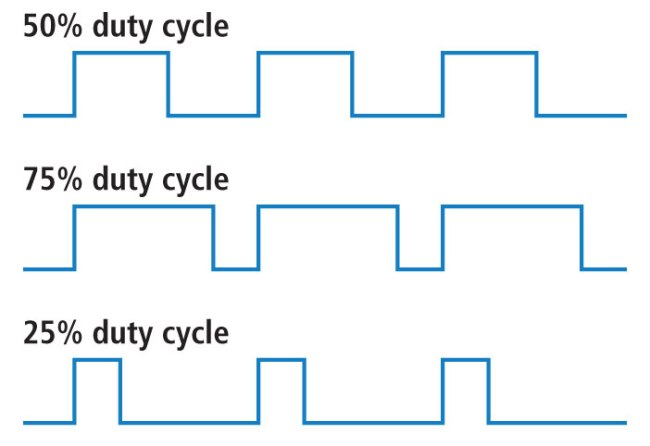
\includegraphics[scale=0.3]{figuras/duty_cycle.jpg}
    \caption{Duty Cycle}
    \label{duty_cycle}
\end{figure}
Em PWM, o tempo em que o sinal fica em nível lógico alto ou baixo não costuma ser muito usado, o mais comum é classificar o sinal de acordo com seu duty-cycle. A relação entre duty-cycle, amplitude e tensão nominal de saída do DAC se torna bem intuitiva. No domínio da frequência, um filtro passa-baixas suprime componentes de alta frequência, consequentemente no domínio do tempo isso acaba "amaciando" o sinal e de certa forma tirando uma media do sinal. Filtrar um sinal PWM com um filtro passa-baixas extrai seu valor médio de tensão. Se por exemplo o duty-cyle de um sinal for 50\% com máximo e mínimo respectivamente em 5 e 0V, após o sinal ser passado pelo filtro o sinal de saída ira possuir uma saída de 2.5V.

\begin{equation}\label{calc-duty-cycle}
    D=\frac{ PW }{ T } \cdot 100 \%
\end{equation}

Na Equação \ref{calc-duty-cycle}, D é o valor do duty cyle em percentagem, PW a largura do pulso e T o período total do sinal.

\begin{equation}\label{calc-analog-voltage}
    V_{out}=\frac{ Pw }{ T } \cdot V_{max}
\end{equation}

A Equação \ref{calc-analog-voltage} calcula a tensão de saída aproximada do sinal após o filtro passa-baixas. Na mesma $V_{out}$ é a tensão de saída, PW a largura do pulso e T o período total do sinal e $V_{max}$ é a tensão do sinal PWM quando em nível lógico alto.

\subsubsection*{Filtro passa-baixas}

Existem duas condições a serem consideradas no projeto do filtro passa-baixas: O tempo de estabilização e o ripple. Tempo de estabilização é o tempo que o sinal leva para chegar ao nível analógico desejado, já o ripple é o ruído residual da filtragem do sinal do saída. Uma frequência de corte baixa gera um sinal com pouco ripple porém aumenta o tempo de estabilização, consequentemente uma frequência de corte mais alta produz um ripple muito grande e um tempo de estabilização curto. O que deve ser feito é escolher uma frequência de corte que gera um ripple menor que a resolução da entrada analógica do inversor de frequência (vale lembrar que resolução é a menor variação de tensão que o dispositivo pode ler). \\

As especificações para projeto do filtro conversor são:

\begin{itemize}
    \item Frequência PWM de entrada = 100KHz
    \item Resolução da entrada do inversor (ripple máximo) = 9.76mV
    \item Tempo de estabilização = 0.1s
    \item Ganho de Tensão = 3
\end{itemize}

O circuito a ser usado será o da Figura \ref{active-lpf}:

\begin{figure}[htbp]
    \centering
    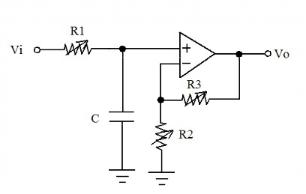
\includegraphics[scale=0.3]{figuras/lpf.jpg}
    \caption{Filtro passa-baixas ativo}
    \label{active-lpf}
\end{figure}

A frequência de corte para o filtro é dada pela Equação \ref{cuttof-frequency}

\begin{equation}\label{cutoff-frequency}
    f_{c}=\frac{ 1 }{ 2 \Pi \cdot R_{1}\cdot C } \cdot V_{max}
\end{equation}

Os resistores $R_{2}$ e $R_{3}$ controlam o ganho do filtro que é dado pela Equação \ref{ganho_alpf}

\begin{equation}\label{calc-analog-voltage}
    G= 1 + \frac{ R_{3} }{ R_{2} }
\end{equation}

Foram usados os seguintes componentes para o circuito:

\begin{itemize}
    \item $R_{1}=10k\Omega$
    \item $R_{2}=100k\Omega$
    \item $R_{3}=200k\Omega$
    \item C=1uF
\end{itemize}

Esse circuito gera uma frequência de corte de aproximadamente 16Hz, um ripple de 2.4mV, um tempo de estabilização de 0.02s e um ganho de tensão igual a 3. Dessa forma atende todas os requisitos de funcionamento. A Figura \ref{filter_out} mostra a saída sem ripple.

\begin{figure}[htbp]
    \centering
    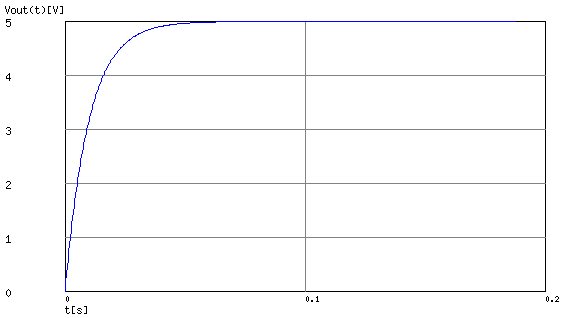
\includegraphics[scale=0.3]{figuras/ripple-lpf.png}
    \caption{Gráfico TensãoxTempo filtro passa baixas}
    \label{filter_out}
\end{figure}



